\documentclass{report}

\usepackage{amsmath}
\usepackage{amssymb}
\usepackage{graphicx}

\newcommand{\dd}{
	\mathop{}\mathopen{}\mathrm{d}
}

\begin{document}
\chapter{Introduction}
\label{chap:intro}

\section{Firing rate models}

-phenomenological, not derived from spiking neuron \cite{DayAbb05}

\section{Renewal spiking neuron model}
\label{sec:renew}

Renewal processes keep memory of the last event, las firing time $\hat{t}$. For those processes the spikes are generated according to a stochastic intensity called the hazard rate
\begin{equation}
  \label{eq:rho1}
\rho(t|\hat{t})=\rho(\tau)
\end{equation}

which depends on the age of the neuron $\tau$, i.e the time since the last spike $\tau=t-\hat{t}$. $\rho(\tau)$ define the probability to spike between $t+\Delta t$ knowing that there were no spike bewteen $t$ and $\hat{t}$

The renewal theory allows to define the probability of the next event given the age of the system, to calculate the interspike-interval (ISI) distribution, i.e the probability to spike at age $\tau$ and no spike before.

\begin{equation}
  \label{eq:P1}
P(\tau)=P(\hat{t}+\tau| \hat{t})
\end{equation}

The ISI distribution satisfy

\begin{equation}
  \label{eq:Pnorm}
\int_0^\infty P(\tau)\dd\tau=1 
\end{equation}

and allows to compute the moment:


\begin{equation}
  \label{eq:Pmoment}
<\tau^n>=\int_0^\infty \tau^nP(\tau)\dd\tau
\end{equation}

Integration of $P(\tau)$ over time yields a probability as the interval distribution $P(\tau)$ is a probability density. The probability that neuron which has fired a spike at $\hat{t}$ and fires the next spike at between $\hat{t}$ and $t$ is given by $\int_0^\tau P(s) \dd s$.

The interspike-interval (ISI) distribution can be linked to the survivor function:
\begin{equation}
  \label{eq:S1}
	S(\tau)=1-\int_0^\tau P(s) \dd s
\end{equation}


The survivor function $S(\tau)$ define the probability that a neuron reach the age $\tau$, so that a neuron "survive" without firing between $\hat{t}$ and $t$.

The hazard rate $\rho(\tau)$ corresponds to the rate of decay of the survivor function:
\begin{equation}
\label{eq:ratedecays}
\rho(\tau)=-\frac{\frac{\dd}{\dd \tau}S(\tau)}{S(\tau)}
\end{equation}

Integrating eq.\ref{eq:ratedecays} yields to the survivor function:
\begin{equation}
  \label{eq:S2}
S(\tau)=\exp\big[-\int_0^\tau\rho(s)\dd s\big]
\end{equation}

Taking the derivative of eq.\eqref{eq:S1}, we can expressed the interspike-interval (ISI) distribution:
\begin{equation}
\label{eq:P2}
P(\tau)=-\frac{\dd}{\dd \tau}S(\tau)=\rho(\tau)S(\tau)
\end{equation}

Eq.\eqref{eq:P2} describe that probability to spike at age $\tau$ and no spike before $P(\tau)$, is given by the product of the probability to survive until age $\tau$ times the momentary hazard $\rho(\tau)$. Inserting eq.\eqref{eq:S2} ineq.\ref{eq:P2} The interval distribution can be explicitly express in terms of the hazard, and is by itself normalized:

\begin{equation}
\label{eq:P2}
P(\tau)=-\frac{\dd}{\dd \tau}S(\tau)=\rho(\tau)\exp\big[-\int_0^\tau\rho(s)\dd s\big]
\end{equation}





\subsection{Examples }
\label{sec:ex}

Interval distribution and hazard functions have been measured in many experiments. Here are some examples widely used.



\subsubsection{Simple model with recovery function}

In the previous section we were implicitly considering stationary renewal system using the notation $\rho(t|\hat{t})$. In this section we will used the notation $\rho(\tau,h)$,with $h$ a time dependent parameter, to show explicitly that$\rho(tau)$ can change in time.


\begin{equation}
  \label{eq:hi}
  \tau_m\dot h=-h+\mu(t)
\end{equation}



Were $mu(t)$ is a time dependent external input.

The hazard rate, can be expressed using a recovery function $g(\tau)$

\begin{equation}
\label{eq:rho}
\rho(\tau,h)=\Phi(h)g(\tau)
\end{equation}

With 

\begin{equation}
\label{eq:phi}
\Phi(h)=\frac{\nu_{max}}{1+\exp[-\beta(h-h_0)]}
\end{equation}

The hazard rate, the survival probability, and the interval distribution are shown in Fig.\ref{fig:renewalprocess} for two Examples of recovery function $g$. Fig.\ref{fig:renewalprocess}(a) corresponds to a poisson process with absolute refractoriness: 
\begin{equation}
\label{eq:poissonabs}
g(\tau)=\theta(\tau-\Delta)
\end{equation}
 The recovery function for Fig.\ref{fig:renewalprocess}(b) is given by
\begin{equation}
\label{eq:expabs}
  g(\tau)=\left[1-\exp(-\lambda(\tau-\Delta))\right]\theta(\tau-\Delta)
\end{equation}

The main difference is that for the poisson neuron with absolute refractoriness the recovery function eq.\eqref{eq:poissonabs} make a jump, whereas in eq.\eqref{eq:expabs} the transition is smooth.
\begin{figure}
(a) \\
	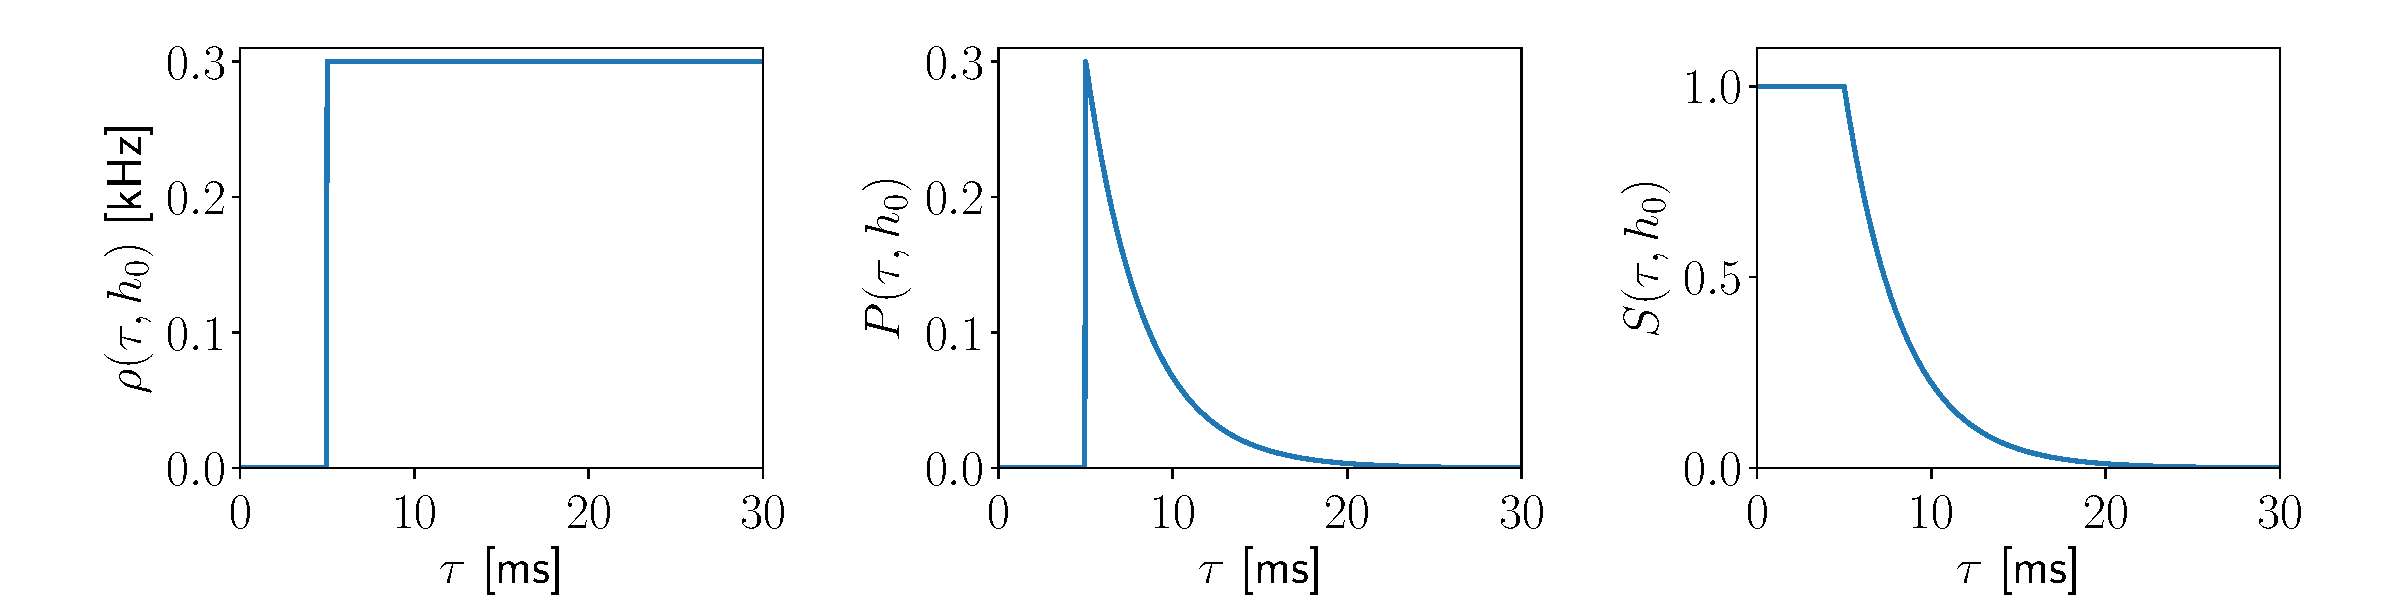
\includegraphics[width=\linewidth]{poissonRHOSP.pdf}
	(b)\\
	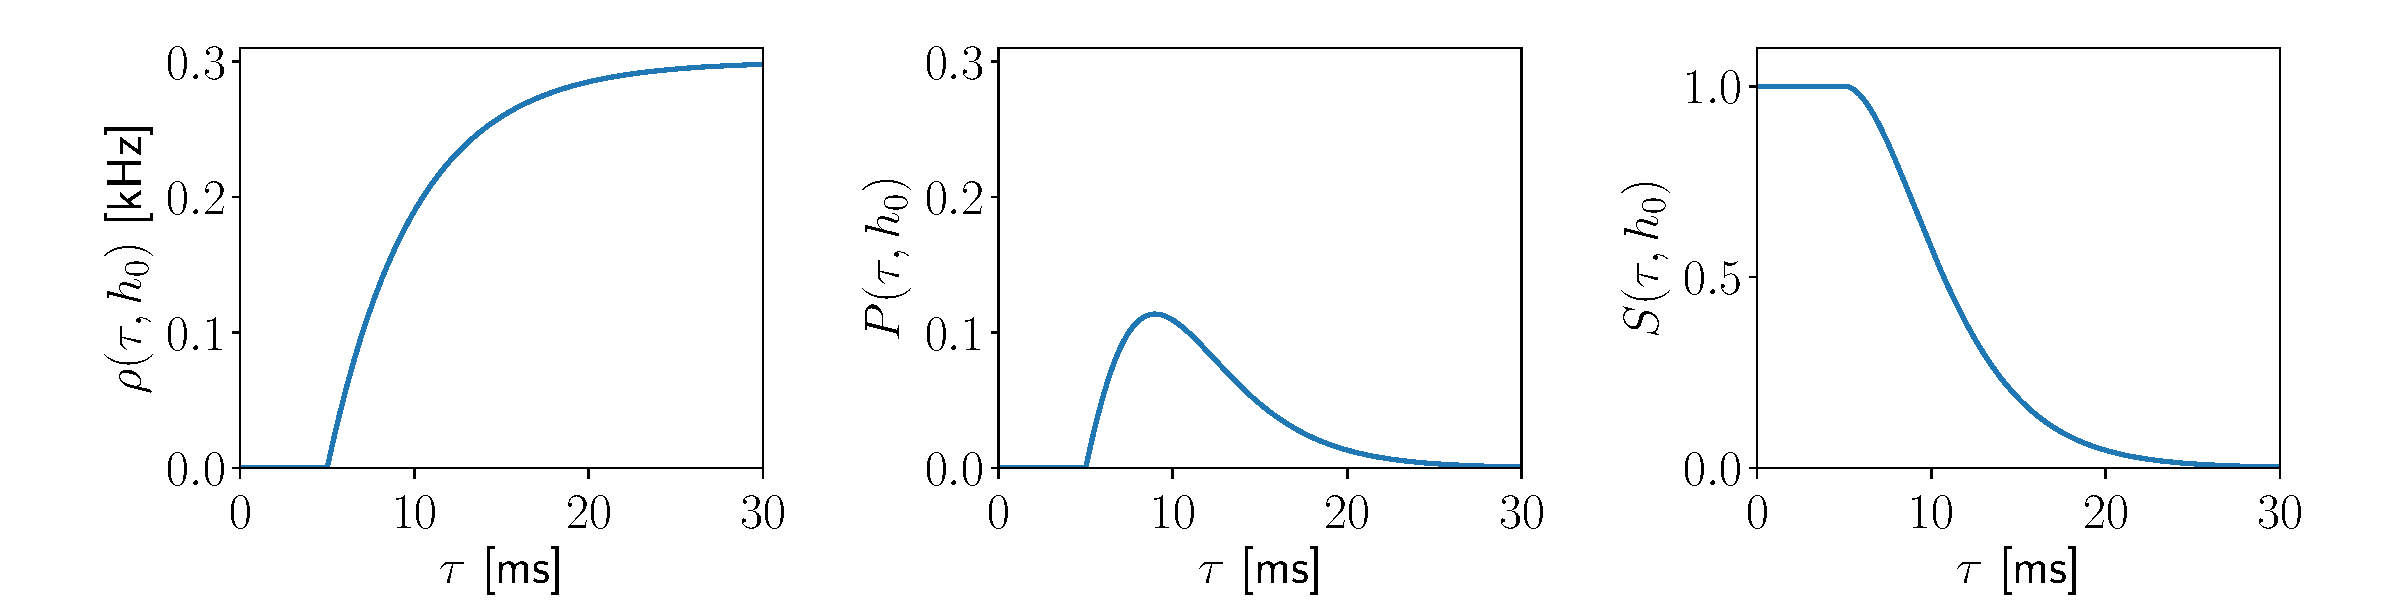
\includegraphics[width=\linewidth]{expRHOSP.pdf}
	\caption{Hazard rate $\rho(\tau,h)$ (left), interval distribution $P(\tau,h)$ (middle) and survivor functio $S(\rho(\tau,h)$ (right) for different recovery function $g(\tau)$. (a) Recovery function corresponds to a Poisson neuron with absolute refractoriness $\Delta$, with $Delta=5$ ms, $h=h_0$, $\nu_{max}=0.6$ kHz.  (b) Recovery function defined  by $ g(\tau)=\left[1-\exp(-\lambda(\tau-\Delta))\right]\theta(\tau-\Delta)$ Poisson neuron with absolute refractoriness $\Delta$, with $\Delta=5$ ms, $h=h_0$, $\nu_{max}=0.6$ kHz.  }
	\label{fig:renewalprocess}
\end{figure}
 

\subsubsection{Gamma process}

$\beta=5$kHz
$\gamma=100$


\begin{figure}

	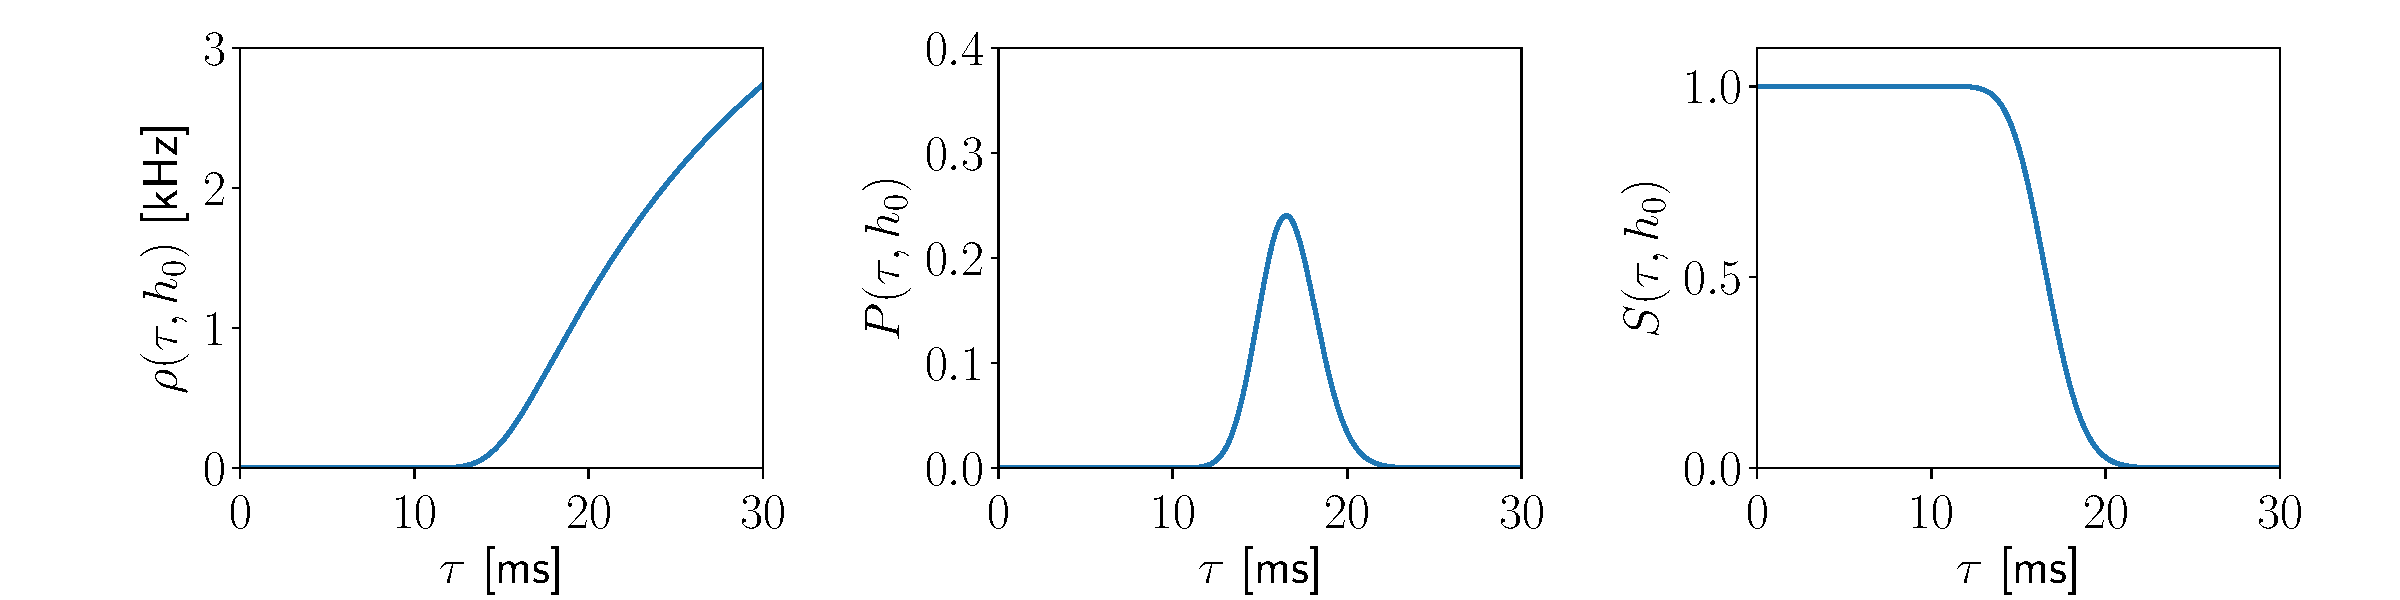
\includegraphics[width=\linewidth]{gamma.pdf}
	\caption{Hazard rate $\rho(\tau)$ (left), interval distribution $P(\tau)$ (middle) and survivor functio $S(\rho(\tau)$ (right) for different recovery function $g(\tau)$. }
	\label{fig:renewalprocess}
\end{figure}

\subsubsection{Perfect integrate-and-fire model driven by white noise}
\label{sec:pif}



\section{Populations of neurons and refractory density equations}


\subsection{Network model}


- population activity definition

- definition of network : all-to-all coupling

-external input $\mu(t)$
\begin{equation}
  \mu(t)=V_{rest}+RI_{ext}(t)+RI_{syn}(t)
\end{equation}

- and/or synaptic input
\begin{equation}
  \label{eq:input}
  RI_{syn}(t)=\tau_mJA(t)
\end{equation}


\section{Spectral decomposition method}

-main idea
- everything known about the method that applies to a general operator L 

-assume that neuron can be described by one state variable, e.g. membrane potential or age. p(v) or q(tau). For concreteness lets consider q(tau)

\subsection{Refractory density equation}

\cite{Ger00,ChiGra07}
-bounary conditions




\subsection{Spectral decomposition for the refractory density equation}


\chapter{Theory}
\label{chap:theo}

-adjoint operator
\subsection{Full Mattia 2002 system}

\section{Low-dimensional dynamics}

\subsection{Truncation Full Mattia 2002 system}

\subsection{Schaffer like}

\subsection{Mattias equation}



\chapter{Spectral properties of specific models}
\label{chap:specif-model}


\section{Poisson neuron with absolute refractoriness}
\label{sec:absref}

\section{Gamma process}

\section{PIF neuron}
\label{sec:pif}


\section{General renewal neuron}
\label{sec:gen-renw}

\chapter{Population response to time-dependent input}

--for uncoupled neurons
--susceptibility

\chapter{Population dynamics of coupled neurons}

- one population

- two populations (E-I net)


\bibliography{my}
\end{document}

%%% Local Variables:
%%% mode: latex
%%% TeX-master: t
%%% End:
